% Options for packages loaded elsewhere
\PassOptionsToPackage{unicode}{hyperref}
\PassOptionsToPackage{hyphens}{url}
%
\documentclass[
]{book}
\usepackage{amsmath,amssymb}
\usepackage{iftex}
\ifPDFTeX
  \usepackage[T1]{fontenc}
  \usepackage[utf8]{inputenc}
  \usepackage{textcomp} % provide euro and other symbols
\else % if luatex or xetex
  \usepackage{unicode-math} % this also loads fontspec
  \defaultfontfeatures{Scale=MatchLowercase}
  \defaultfontfeatures[\rmfamily]{Ligatures=TeX,Scale=1}
\fi
\usepackage{lmodern}
\ifPDFTeX\else
  % xetex/luatex font selection
\fi
% Use upquote if available, for straight quotes in verbatim environments
\IfFileExists{upquote.sty}{\usepackage{upquote}}{}
\IfFileExists{microtype.sty}{% use microtype if available
  \usepackage[]{microtype}
  \UseMicrotypeSet[protrusion]{basicmath} % disable protrusion for tt fonts
}{}
\makeatletter
\@ifundefined{KOMAClassName}{% if non-KOMA class
  \IfFileExists{parskip.sty}{%
    \usepackage{parskip}
  }{% else
    \setlength{\parindent}{0pt}
    \setlength{\parskip}{6pt plus 2pt minus 1pt}}
}{% if KOMA class
  \KOMAoptions{parskip=half}}
\makeatother
\usepackage{xcolor}
\usepackage{color}
\usepackage{fancyvrb}
\newcommand{\VerbBar}{|}
\newcommand{\VERB}{\Verb[commandchars=\\\{\}]}
\DefineVerbatimEnvironment{Highlighting}{Verbatim}{commandchars=\\\{\}}
% Add ',fontsize=\small' for more characters per line
\usepackage{framed}
\definecolor{shadecolor}{RGB}{248,248,248}
\newenvironment{Shaded}{\begin{snugshade}}{\end{snugshade}}
\newcommand{\AlertTok}[1]{\textcolor[rgb]{0.94,0.16,0.16}{#1}}
\newcommand{\AnnotationTok}[1]{\textcolor[rgb]{0.56,0.35,0.01}{\textbf{\textit{#1}}}}
\newcommand{\AttributeTok}[1]{\textcolor[rgb]{0.13,0.29,0.53}{#1}}
\newcommand{\BaseNTok}[1]{\textcolor[rgb]{0.00,0.00,0.81}{#1}}
\newcommand{\BuiltInTok}[1]{#1}
\newcommand{\CharTok}[1]{\textcolor[rgb]{0.31,0.60,0.02}{#1}}
\newcommand{\CommentTok}[1]{\textcolor[rgb]{0.56,0.35,0.01}{\textit{#1}}}
\newcommand{\CommentVarTok}[1]{\textcolor[rgb]{0.56,0.35,0.01}{\textbf{\textit{#1}}}}
\newcommand{\ConstantTok}[1]{\textcolor[rgb]{0.56,0.35,0.01}{#1}}
\newcommand{\ControlFlowTok}[1]{\textcolor[rgb]{0.13,0.29,0.53}{\textbf{#1}}}
\newcommand{\DataTypeTok}[1]{\textcolor[rgb]{0.13,0.29,0.53}{#1}}
\newcommand{\DecValTok}[1]{\textcolor[rgb]{0.00,0.00,0.81}{#1}}
\newcommand{\DocumentationTok}[1]{\textcolor[rgb]{0.56,0.35,0.01}{\textbf{\textit{#1}}}}
\newcommand{\ErrorTok}[1]{\textcolor[rgb]{0.64,0.00,0.00}{\textbf{#1}}}
\newcommand{\ExtensionTok}[1]{#1}
\newcommand{\FloatTok}[1]{\textcolor[rgb]{0.00,0.00,0.81}{#1}}
\newcommand{\FunctionTok}[1]{\textcolor[rgb]{0.13,0.29,0.53}{\textbf{#1}}}
\newcommand{\ImportTok}[1]{#1}
\newcommand{\InformationTok}[1]{\textcolor[rgb]{0.56,0.35,0.01}{\textbf{\textit{#1}}}}
\newcommand{\KeywordTok}[1]{\textcolor[rgb]{0.13,0.29,0.53}{\textbf{#1}}}
\newcommand{\NormalTok}[1]{#1}
\newcommand{\OperatorTok}[1]{\textcolor[rgb]{0.81,0.36,0.00}{\textbf{#1}}}
\newcommand{\OtherTok}[1]{\textcolor[rgb]{0.56,0.35,0.01}{#1}}
\newcommand{\PreprocessorTok}[1]{\textcolor[rgb]{0.56,0.35,0.01}{\textit{#1}}}
\newcommand{\RegionMarkerTok}[1]{#1}
\newcommand{\SpecialCharTok}[1]{\textcolor[rgb]{0.81,0.36,0.00}{\textbf{#1}}}
\newcommand{\SpecialStringTok}[1]{\textcolor[rgb]{0.31,0.60,0.02}{#1}}
\newcommand{\StringTok}[1]{\textcolor[rgb]{0.31,0.60,0.02}{#1}}
\newcommand{\VariableTok}[1]{\textcolor[rgb]{0.00,0.00,0.00}{#1}}
\newcommand{\VerbatimStringTok}[1]{\textcolor[rgb]{0.31,0.60,0.02}{#1}}
\newcommand{\WarningTok}[1]{\textcolor[rgb]{0.56,0.35,0.01}{\textbf{\textit{#1}}}}
\usepackage{longtable,booktabs,array}
\usepackage{calc} % for calculating minipage widths
% Correct order of tables after \paragraph or \subparagraph
\usepackage{etoolbox}
\makeatletter
\patchcmd\longtable{\par}{\if@noskipsec\mbox{}\fi\par}{}{}
\makeatother
% Allow footnotes in longtable head/foot
\IfFileExists{footnotehyper.sty}{\usepackage{footnotehyper}}{\usepackage{footnote}}
\makesavenoteenv{longtable}
\usepackage{graphicx}
\makeatletter
\newsavebox\pandoc@box
\newcommand*\pandocbounded[1]{% scales image to fit in text height/width
  \sbox\pandoc@box{#1}%
  \Gscale@div\@tempa{\textheight}{\dimexpr\ht\pandoc@box+\dp\pandoc@box\relax}%
  \Gscale@div\@tempb{\linewidth}{\wd\pandoc@box}%
  \ifdim\@tempb\p@<\@tempa\p@\let\@tempa\@tempb\fi% select the smaller of both
  \ifdim\@tempa\p@<\p@\scalebox{\@tempa}{\usebox\pandoc@box}%
  \else\usebox{\pandoc@box}%
  \fi%
}
% Set default figure placement to htbp
\def\fps@figure{htbp}
\makeatother
\setlength{\emergencystretch}{3em} % prevent overfull lines
\providecommand{\tightlist}{%
  \setlength{\itemsep}{0pt}\setlength{\parskip}{0pt}}
\setcounter{secnumdepth}{5}
\usepackage{booktabs}
\usepackage{bookmark}
\IfFileExists{xurl.sty}{\usepackage{xurl}}{} % add URL line breaks if available
\urlstyle{same}
\hypersetup{
  pdftitle={Formation R},
  pdfauthor={Benoît Lepage},
  hidelinks,
  pdfcreator={LaTeX via pandoc}}

\title{Formation R}
\author{Benoît Lepage}
\date{2025-07-04}

\begin{document}
\maketitle

{
\setcounter{tocdepth}{1}
\tableofcontents
}
\chapter{Bienvenue sur cette formation au logiciel R}\label{bienvenue-sur-cette-formation-au-logiciel-r}

R est un logiciel accessible gratuitement permettant de réaliser des analyses statistiques dans un environnement windows, macOS ou Linux.

\section{Pourquoi choisir R ?}\label{pourquoi-choisir-r}

Le logiciel est gratuit, très complet, avec une communauté d'utilisateurs très active dans le monde entier. Il est fréquent que les nouvelles méthodes d'analyses statistiques développées dans les équipes académiques soient d'abord mises à disposition sur R.

Le logiciel R repose sur l'utilisation de \textbf{scripts} dans lesquels nous allons \textbf{programmer} les analyses statistiques. Cette écriture sous forme de programmation peut paraître austère à première vue, mais est indispensable pour permettre la \textbf{reproductibilité} et la \textbf{transparence} des analyses. La même démarche de programmation est utilisée dans tous les logiciels statistiques professionnels (Stata, SAS, Python, Matlab, etc).

Pour utiliser R, les premières choses à faire sont de :

\begin{itemize}
\tightlist
\item
  télécharger le logiciel R
\item
  et télécharger un Environnement de Développement Intégré (IDE) comme RStudio.
\end{itemize}

\section{Téléchargez le logiciel R}\label{tuxe9luxe9chargez-le-logiciel-r}

Vous pouvez télécharger la dernière version stable du logiciel R sur le site du \href{https://www.r-project.org/}{R project}.

\begin{figure}

{\centering 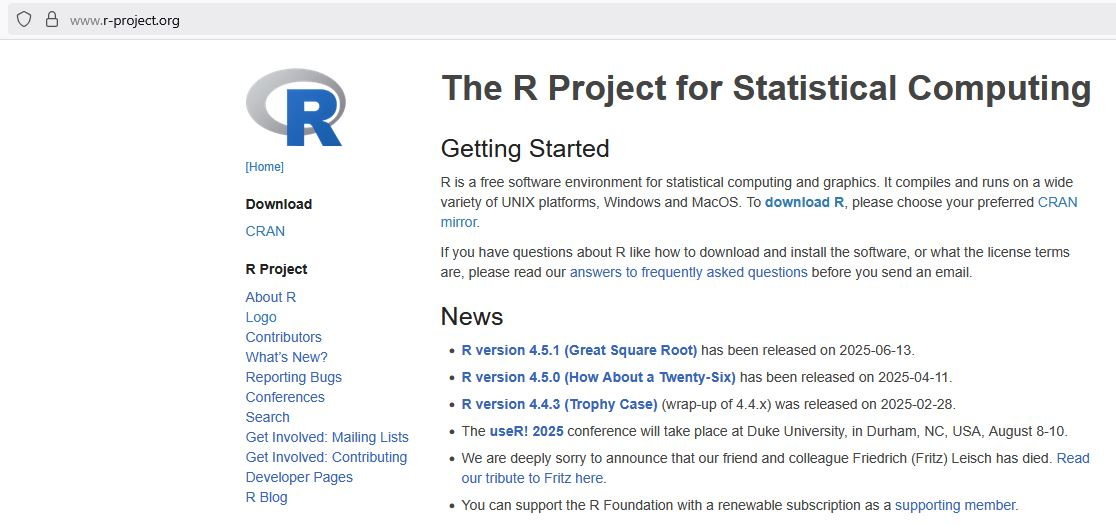
\includegraphics[width=1\linewidth]{./images/telecharger_R_1} 

}

\caption{Site du R project, en juillet 2025}\label{fig:dlR1}
\end{figure}

Cliquez sur ``download R'', choisissez un site mirroir (par exemple un des sites en France).

Puis téléchargez la version de R en fonction de votre système d'exploitation (Windows, macOS ou Linux).

\begin{figure}

{\centering 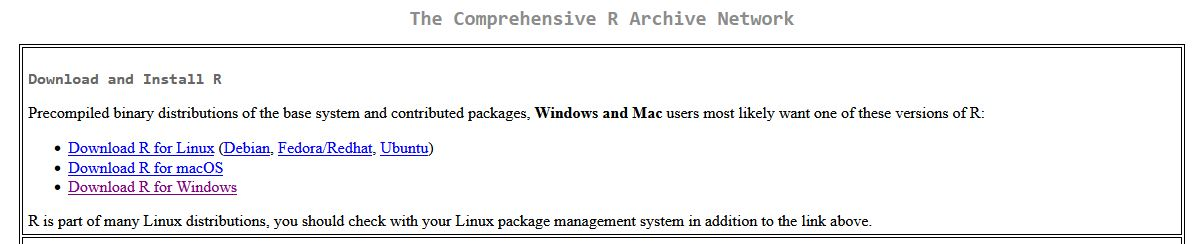
\includegraphics[width=1\linewidth]{./images/telecharger_R_2} 

}

\caption{Choisissez la version adaptée à votre système d'exploitation}\label{fig:dlR2}
\end{figure}

Enfin, installez R à partir du fichier d'installation que vous venez de télécharger.

\subsection{Ouvrez le logiciel R}\label{ouvrez-le-logiciel-r}

Si vous ouvrez le logiciel R, vous aller trouver l'interface graphique de R (\emph{RGui} pour \emph{R Graphical user interface}). Il est possible de faire vos analyses statistiques à partir de cette interface graphique, mais elle est très très austère.

\begin{figure}

{\centering 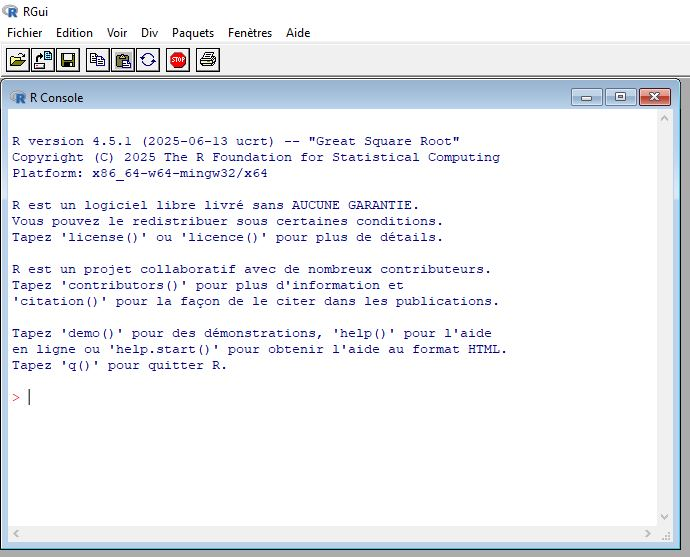
\includegraphics[width=0.5\linewidth]{./images/Rgui} 

}

\caption{L'interface graphique de R (RGui)}\label{fig:RGui}
\end{figure}

Plutôt que d'utiliser cette interface RGui, nous vous recommandons fortement d'utiliser un Environnement de Développement Intégré (IDE), comme RStudio, qui vous facilitera grandement la vie pour utiliser un logiciel statistique qui repose sur de la programmation.

\section{Téléchargez un IDE (RStudio recommandé)}\label{tuxe9luxe9chargez-un-ide-rstudio-recommanduxe9}

RStudio est un environnement qui permet d'utiliser R, mais également d'autres logiciels de programmation comme Python, SQL, Stan, C++, etc. Cet environnement vous facilitera le travail pour :

\begin{itemize}
\tightlist
\item
  éditer vos scripts de programmation,
\item
  accéder à la console,
\item
  visualiser vos environnements de travail avec les fichiers et les objets qu'il contient,
\item
  visualiser vos sorties graphiques et certaines tables d'analyses,
\item
  visualiser vos données,
\item
  visualiser les fichiers d'aide,
\item
  gérer les \emph{packages} permettant de faire des analyses spécifiques,
\item
  et bien d'autres choses encore.
\end{itemize}

Par exemple, le tutoriel que vous êtes en train de lire a été créé à partir du package \href{https://bookdown.org/}{\texttt{bookdown}} avec le logiciels R, au sein de l'IDE RStudio,

Vous pouvez télécharger la dernière version de \href{https://posit.co/download/rstudio-desktop/}{RStudio} sur le site de la compagnie \href{https://posit.co/products/open-source/rstudio/?sid=1}{Posit}. Choisissez la version qui est adaptée à votre système d'exploitation (Windows, macOS ou Linux).

\begin{figure}

{\centering 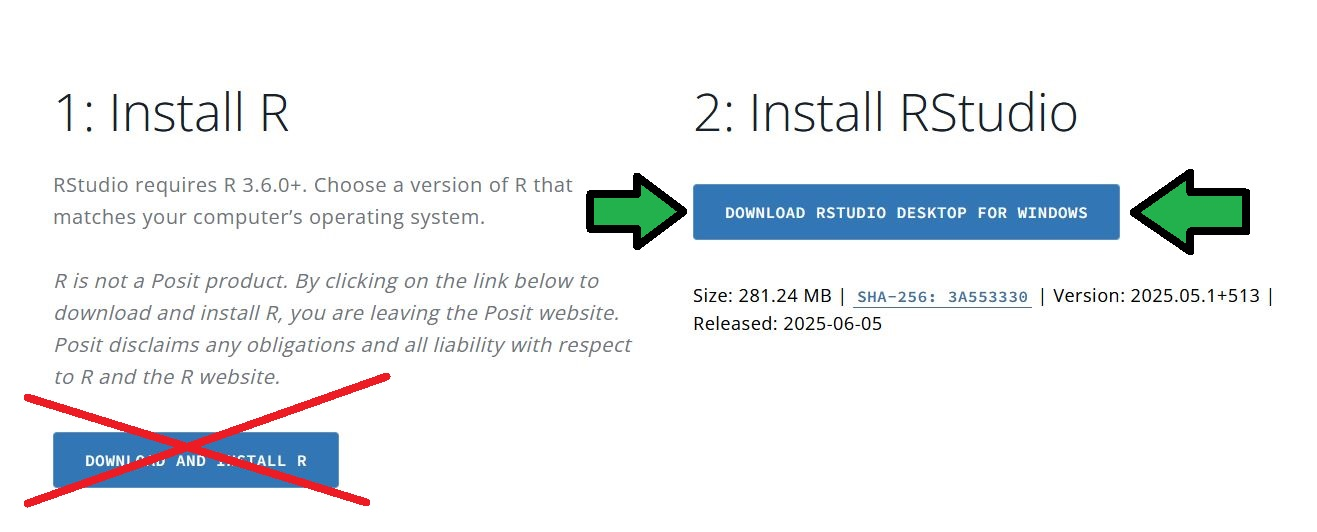
\includegraphics[width=1\linewidth]{./images/telecharger_RStudio_1} 

}

\caption{téléchargez RStudio}\label{fig:dlRStudio-1}
\end{figure}
\begin{figure}

{\centering 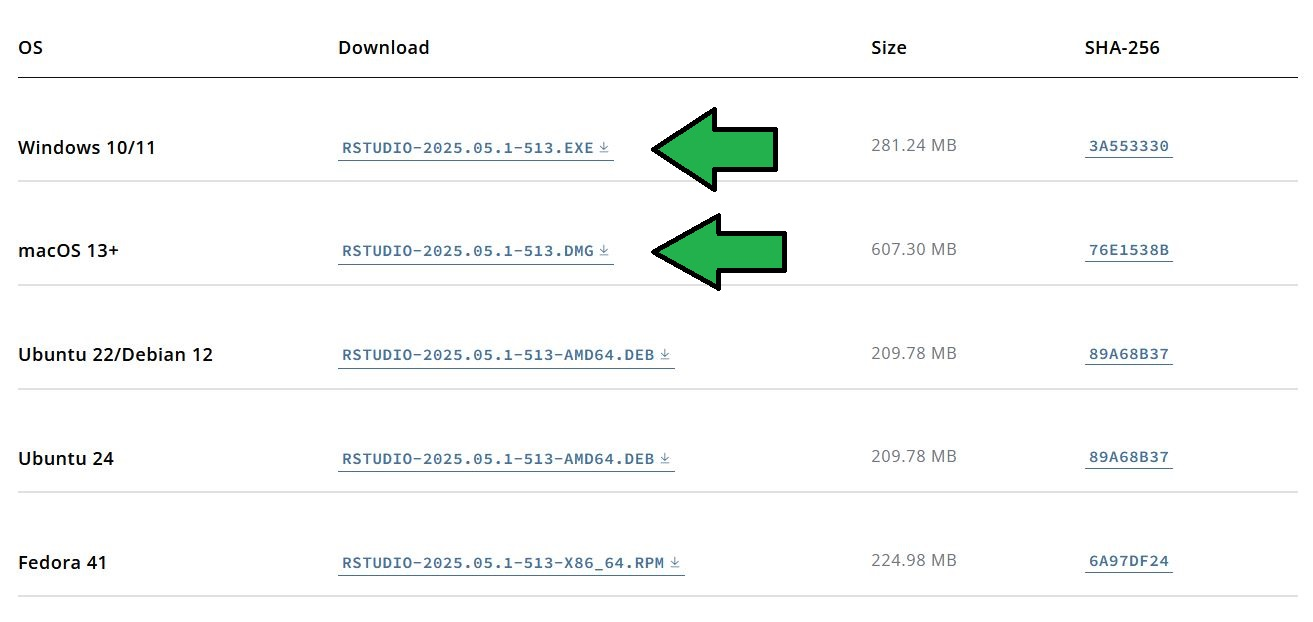
\includegraphics[width=1\linewidth]{./images/telecharger_RStudio_2} 

}

\caption{téléchargez RStudio}\label{fig:dlRStudio-2}
\end{figure}

Puis, installez RStudio à partir du fichier d'installation que vous venez de télécharger.

\subsection{Ouvrez l'IDE RStudio}\label{ouvrez-lide-rstudio}

Ouvrez RStudio, puis commencez par ouvrir un \textbf{script}

\begin{itemize}
\tightlist
\item
  à partir du menu File \textgreater{} New File \textgreater{} R script
\item
  ou bien en utilisant le raccourci Ctrl+Maj+N sur windows
\item
  ou bien en cliquant sur le petit fichier blanc avec un + vert en haut à gauche, puis choisir ``R script''
\end{itemize}

\begin{figure}

{\centering 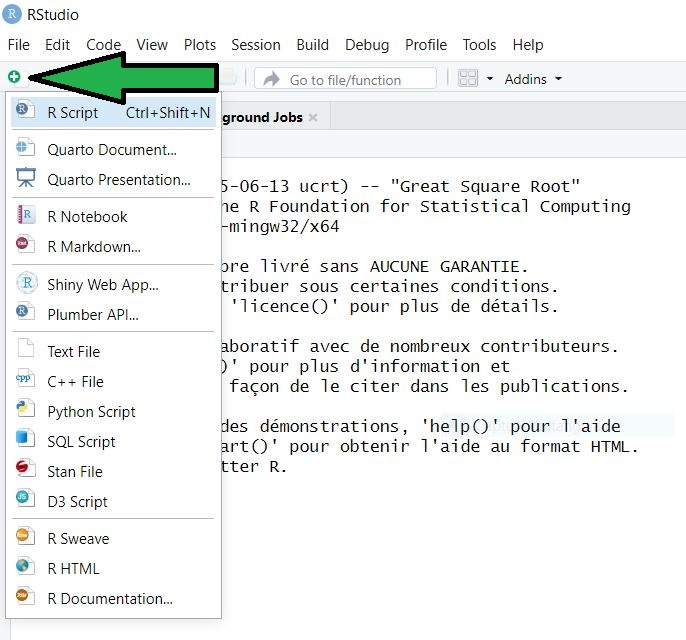
\includegraphics[width=0.5\linewidth]{./images/newscriptR} 

}

\caption{Ouvrir un nouveau script}\label{fig:newscript}
\end{figure}

L'interface de RStudio contient un menu, 4 quadrants et des sous-menus et boutons dans chaque cadrant.

\begin{figure}

{\centering 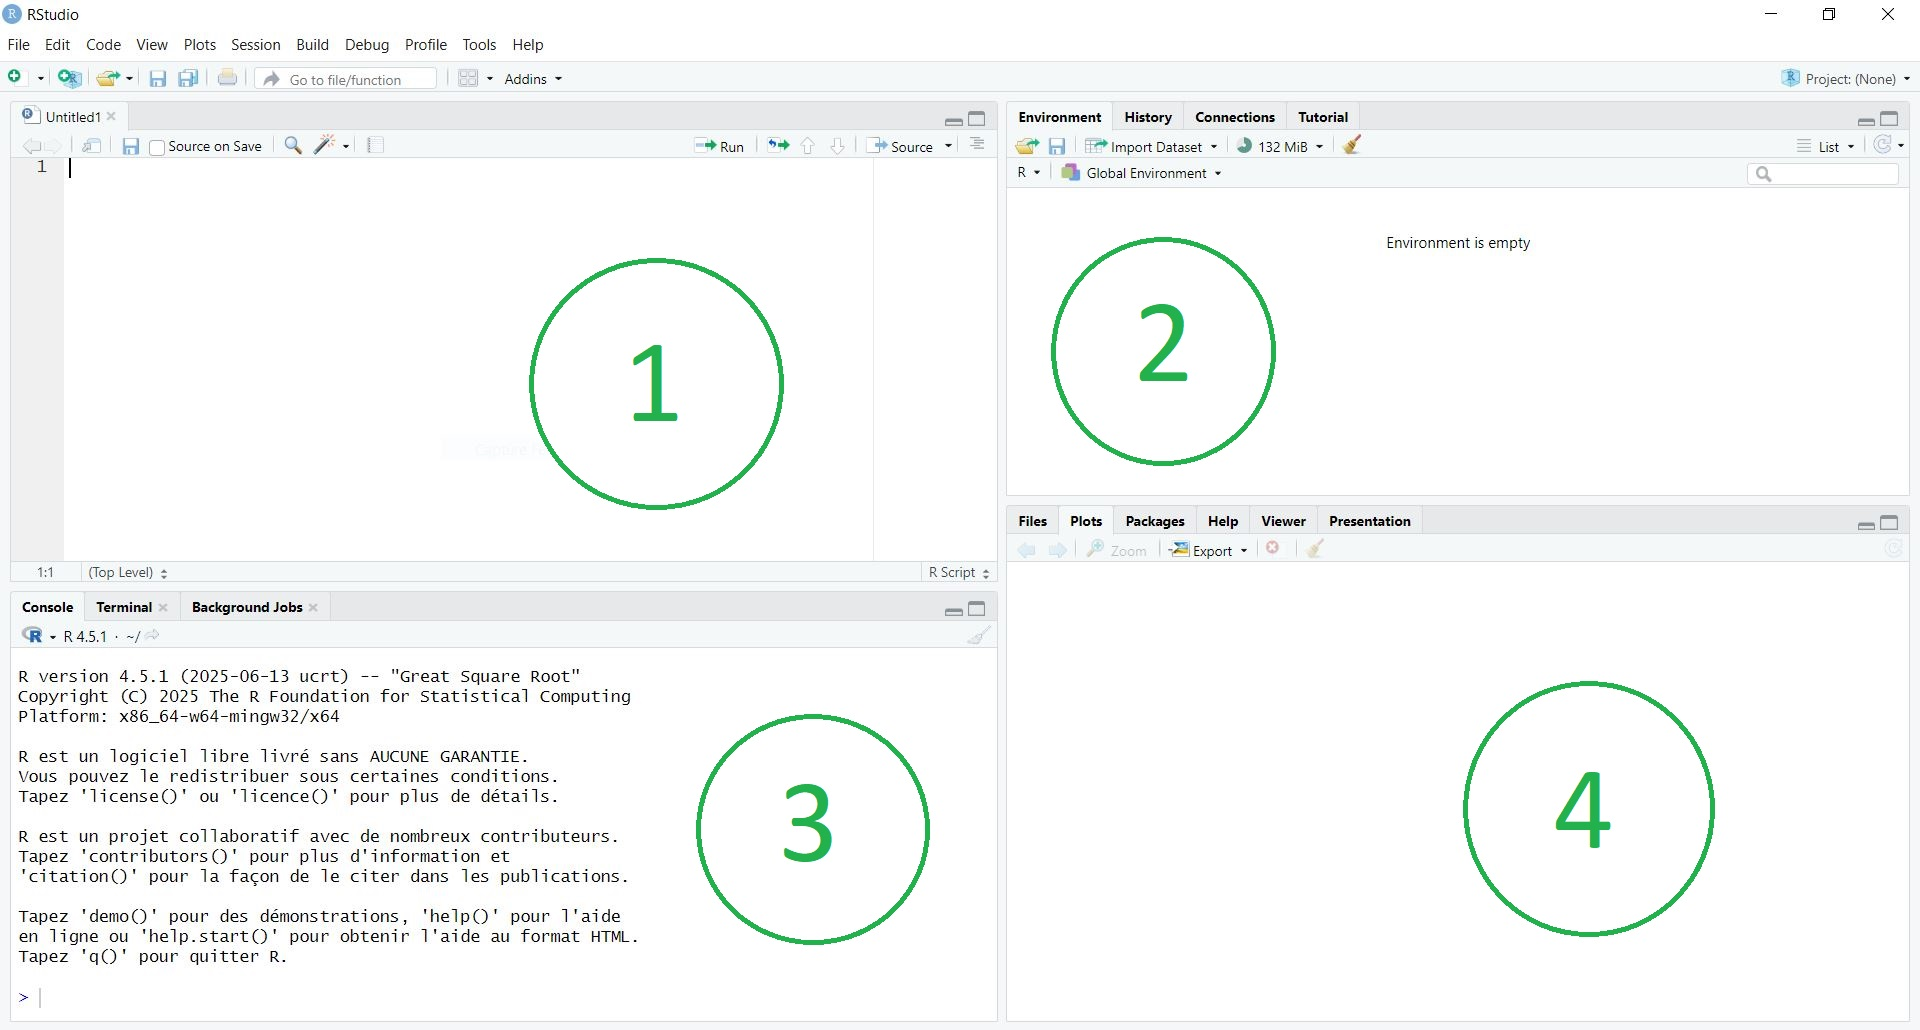
\includegraphics[width=1\linewidth]{./images/cadrants_RStudio} 

}

\caption{Les 4 cadrants de RStudio}\label{fig:RStudcadrants}
\end{figure}

Les menus qui vous seront le plus utiles sont :

\begin{itemize}
\tightlist
\item
  Dans le menu principal,

  \begin{itemize}
  \tightlist
  \item
    le menu \emph{File} vous permettra de créer de nouveaux fichiers, d'ouvrir des fichiers déjà existants, de sauver vos fichiers, d'importer des bases de données, etc.
  \item
    le menu \emph{Tools \textgreater{} Install packages\ldots{}} pour installer de nouveaux packages
  \item
    le menu \emph{Tools \textgreater{} Global Options\ldots{}} vous permet de choisir la version du logiciel R à utiliser (onglet ``R General'') ou bien de changer l'aspect graphique de l'environnement RStudio (onglet ``Appearance'', puis choisissez un ``Editor theme'', avec différentes interfaces claires ou sombres)
  \end{itemize}
\item
  Au sein du \textbf{script} (cadrant 1)

  \begin{itemize}
  \tightlist
  \item
    le bouton ``disquette'' permet de sauvegarder votre script
  \item
    le bouton ``run'' permet de faire tourner votre programme d'analyse (les lignes que vous avez sélectionnées). Par exemple, tapez la commande suivante dans le script, sélectionnez la ligne et cliquez sur le bouton ``run''.
  \end{itemize}
\end{itemize}

\begin{Shaded}
\begin{Highlighting}[]
\FunctionTok{print}\NormalTok{(}\StringTok{"Hello Toulouse"}\NormalTok{)}
\end{Highlighting}
\end{Shaded}

et vous devriez voir la commande \texttt{\textgreater{}\ print("Hello\ Toulouse")} puis son résultat \texttt{"Hello\ Toulouse"} dans l'onglet \textbf{console} du cadrant 3.

\begin{itemize}
\tightlist
\item
  Au sein du cadrant 3, l'onglet le plus utile pour pour les débutants est l'onglet \textbf{console}

  \begin{itemize}
  \tightlist
  \item
    la console est la même que la console affichée dans l'interface RGui du logiciel R que l'on a vu au paragraphe 1.2.1.
  \item
    la console commence par afficher la version de R en cours d'utilisation
  \item
    vous pouvez y saisir des commandes et obtenir directement leurs résultats, par exemple si vous tapez dans la console \texttt{4+9}, vous obtiendrez directement le résultat \texttt{13}. \textbf{Attention, les commandes que vous saisissez directement dans la console ne seront pas sauvegardées. Si vous voulez sauvegarder des commandes, il faut utiliser le \emph{script} (cadrant 1)}
  \end{itemize}
\end{itemize}

\begin{Shaded}
\begin{Highlighting}[]
\DecValTok{4}\SpecialCharTok{+}\DecValTok{9}
\end{Highlighting}
\end{Shaded}

\begin{verbatim}
## [1] 13
\end{verbatim}

\begin{itemize}
\tightlist
\item
  Au sein du cadrant 2, l'onglet le plus utile pour les débutants est l'onglet \textbf{Environment}

  \begin{itemize}
  \tightlist
  \item
    cet onglet vous permettra de visualiser les ``objets R'' créés pendant vos analyses.
  \item
    Par exemple si vous saisissez \texttt{v\ \textless{}-\ 1:10} dans la console, vous allez voir apparaître l'objet \texttt{v} dans l'environnement de travail (il s'agit d'un vecteur de 1 à 10, nommé ``v'').
  \end{itemize}
\item
  Au sein du cadrant 4, les onglets les plus utiles pour les débutants sont :

  \begin{itemize}
  \tightlist
  \item
    l'onglet ``File'' qui contient les dossiers et fichiers au sein d'un dossier de travail (voir le chapitre 3 pour créer et organiser un dossier de travail associé à un ``projet R'')
  \item
    l'onglet ``Plots'' où vous retrouverez vos sorties graphiques. Au sein de cet onglet, vous trouverez un menu pour exporter vos graphiques selon différents formats. Des boutons permettent également de zoomer et d'effacer les graphiques. Par exemple, si vous saisissez \texttt{hist(rnorm(10000))} dans la console, un histogramme d'une distribution normale centrée réduite va apparaître. Vous pouvez effacer la figure en cliquant sur le bouton avec la croix rouge (efface la figure actuelle) ou le balet (efface l'ensemble des figures).
  \item
    l'onglet ``Packages'' où vous pourrez activer, désactiver ou mettre à jour les packages qui ont été téléchargés.
  \item
    l'onglet ``Help'' où vous trouverez de l'aide. Par exemple si vous saisissez \texttt{help(mean)} dans la console, l'aide de la commande \texttt{mean} va s'afficher. Vous pouvez également utiliser le champ de recherche de fonctions dans le menu ``Help''.
  \end{itemize}
\end{itemize}

\end{document}
